% Gabarit pandoc des corrigés publiés (brut et guidé). Contenu sans marque ni nom de site.
% Compilation : lualatex (latexmk -lualatex).
% Le Markdown reste la source unique : ne pas éditer ce fichier .tex à la main.
\documentclass[11pt,a4paper]{article}

% --- Moteur, polices (Latin Modern) et langue ---------------------------------
\usepackage{iftex}
\ifLuaTeX\else\errmessage{Ce document se compile avec lualatex}\fi
\usepackage{amsmath,amssymb,mathtools}
\usepackage{fontspec}
% mathrm=sym : \mathrm prend ses glyphes dans la police mathématique (ℓ, μ, Ω), comme KaTeX.
\usepackage[math-style=TeX,bold-style=TeX,mathrm=sym]{unicode-math}
% Repli pour les glyphes absents de Latin Modern (indices et exposants Unicode,
% flèches, filets des schémas en texte, symboles) : DejaVu, puis Latin Modern Math
% (ℓ, lettres mathématiques Unicode des légendes).
\directlua{
  luaotfload.add_fallback("repliTexte", {"DejaVuSerif:mode=harf;", "DejaVuSans:mode=harf;", "file:latinmodern-math.otf:mode=harf;"})
  luaotfload.add_fallback("repliMono", {"DejaVuSansMono:mode=harf;", "DejaVuSans:mode=harf;", "file:latinmodern-math.otf:mode=harf;"})
}
\setmainfont{Latin Modern Roman}[RawFeature={fallback=repliTexte}]
\setsansfont{Latin Modern Sans}[RawFeature={fallback=repliTexte}]
\setmonofont{Latin Modern Mono}[RawFeature={fallback=repliMono}]
\setmathfont{Latin Modern Math}
\usepackage[french]{babel}
\frenchsetup{SmallCapsFigTabCaptions=false}

% --- Mise en page --------------------------------------------------------------
\usepackage[a4paper,margin=2.2cm,headheight=14pt,footskip=1.2cm]{geometry}
\usepackage{microtype}
\setlength{\emergencystretch}{4em}
\tolerance=1500
\setlength{\parindent}{0pt}
\setlength{\parskip}{0.55\baselineskip plus 2pt minus 1pt}
\usepackage{xcolor}
% Gris nommés : babel-french rend « ! » actif dans le document.
\definecolor{gris2}{gray}{0.98}
\definecolor{gris3}{gray}{0.97}
\definecolor{gris5}{gray}{0.95}
\definecolor{gris35}{gray}{0.65}
\definecolor{gris40}{gray}{0.60}
\definecolor{gris45}{gray}{0.55}
\definecolor{gris50}{gray}{0.50}
\definecolor{gris55}{gray}{0.45}
\definecolor{gris60}{gray}{0.40}
\definecolor{gris65}{gray}{0.35}
\definecolor{gris70}{gray}{0.30}
\definecolor{gris80}{gray}{0.20}
\definecolor{gris85}{gray}{0.15}
\usepackage{graphicx}
\usepackage{float}
\usepackage{caption}
\captionsetup{font=small,labelformat=empty,justification=centering}
\usepackage{booktabs,longtable,array,multirow,calc}
\usepackage{siunitx}
\sisetup{locale=FR}
\usepackage[version=4]{mhchem}
\usepackage{listings}
\usepackage{fancyhdr}
\usepackage{lastpage}
\usepackage[most]{tcolorbox}
\usepackage{enumitem}
\setlist{nosep,leftmargin=*,topsep=2pt}
\usepackage[hidelinks,unicode]{hyperref}
\usepackage{bookmark}
\hypersetup{pdftitle={Banque PT — Mathématiques B 2026},pdfauthor={Rédigé par IA},pdfcreator={LaTeX},pdfsubject={Corrigé brut}}
\usepackage{xurl}

% --- Pandoc : listes, tableaux, figures ----------------------------------------
\providecommand{\passthrough}[1]{#1}
\providecommand{\tightlist}{\setlength{\itemsep}{0pt}\setlength{\parskip}{0pt}}

\makeatletter
\def\maxwidth{\ifdim\Gin@nat@width>\linewidth\linewidth\else\Gin@nat@width\fi}
\def\maxheight{\ifdim\Gin@nat@height>0.55\textheight 0.55\textheight\else\Gin@nat@height\fi}
\makeatother
\setkeys{Gin}{width=\maxwidth,height=\maxheight,keepaspectratio}
\setcounter{secnumdepth}{-\maxdimen}
\providecommand{\pandocbounded}[1]{#1}

% --- Code (listings) -----------------------------------------------------------
\lstset{
  basicstyle=\ttfamily\small,
  columns=fullflexible,
  keepspaces=true,
  breaklines=true,
  breakatwhitespace=false,
  postbreak=\mbox{\textcolor{gris50}{$\hookrightarrow$}\space},
  frame=single,
  rulecolor=\color{gris35},
  framesep=4pt,
  xleftmargin=5pt,xrightmargin=5pt,
  backgroundcolor=\color{gris3},
  keywordstyle=\bfseries,
  commentstyle=\color{gris65},
  stringstyle=\color{gris80},
  showstringspaces=false,
  tabsize=4,
  extendedchars=true,
  aboveskip=6pt,belowskip=6pt,
}

% --- Macros des corrigés (KaTeX ↔ LaTeX) ---------------------------------------
% Les corrigés sont écrits pour KaTeX : on définit ici ce que KaTeX connaît et
% que LaTeX n'a pas, sans jamais retoucher le Markdown.
\providecommand{\R}{\mathbb{R}}
\providecommand{\N}{\mathbb{N}}
\providecommand{\Z}{\mathbb{Z}}
\providecommand{\Q}{\mathbb{Q}}
\providecommand{\C}{\mathbb{C}}
\providecommand{\dd}{\mathrm{d}}
\providecommand{\llbracket}{\lBrack}
\providecommand{\rrbracket}{\rBrack}
\providecommand{\lBrace}{\lbrace}
\providecommand{\rBrace}{\rbrace}
\providecommand{\Box}{\square}
\providecommand{\Diamond}{\lozenge}
\providecommand{\varnothing}{\emptyset}
\providecommand{\argmax}{\operatorname*{arg\,max}}
\providecommand{\argmin}{\operatorname*{arg\,min}}
\renewcommand{\leq}{\leqslant}
\renewcommand{\geq}{\geqslant}

% Équation hors texte : réduite à la largeur de la ligne si elle déborde.
\newsavebox{\boiteequation}
\newcommand{\equationajustee}[1]{%
  \sbox{\boiteequation}{$\displaystyle #1$}%
  \ifdim\wd\boiteequation>\linewidth
    \[\resizebox{\linewidth}{!}{\usebox{\boiteequation}}\]%
  \else
    \[#1\]%
  \fi}

% --- Encadrés pédagogiques (sobres, lisibles en noir et blanc) -----------------
\tcbset{
  encadre/.style={
    enhanced,breakable,sharp corners,
    colback=white,colframe=gris55,
    boxrule=0.4pt,leftrule=2.2pt,
    left=6pt,right=6pt,top=3pt,bottom=3pt,
    before skip=6pt,after skip=6pt,
    fonttitle=\bfseries\small,coltitle=black,
    attach title to upper,after title={\quad},
    parbox=false,
  }
}
\newtcolorbox{indication}[1]{encadre,colframe=gris45,colback=gris2,title={Indication~#1}}
\newtcolorbox{methode}{encadre,colframe=gris70,title={Méthode}}
\newtcolorbox{piege}{encadre,colframe=gris85,boxrule=0.8pt,leftrule=2.2pt,title={Piège}}
\newtcolorbox{jury}{encadre,colframe=gris60,colback=gris5,title={Jury}}
\newtcolorbox{encadrenote}{encadre,colframe=gris40}

% --- Titres de section ---------------------------------------------------------
\usepackage{titlesec}
\titleformat{\section}{\Large\bfseries}{}{0pt}{}
\titleformat{\subsection}{\large\bfseries}{}{0pt}{}
\titleformat{\subsubsection}{\normalsize\bfseries}{}{0pt}{}
\titlespacing*{\section}{0pt}{14pt plus 4pt minus 2pt}{6pt}
\titlespacing*{\subsection}{0pt}{10pt plus 3pt minus 2pt}{4pt}
\titlespacing*{\subsubsection}{0pt}{8pt plus 2pt minus 2pt}{2pt}

% --- En-tête et pied de page ---------------------------------------------------
\pagestyle{fancy}
\fancyhf{}
\fancyhead[L]{\small\textsc{Corrigé brut} · Banque PT PT}
\fancyhead[R]{\small Maths B 2026}
\fancyfoot[L]{\footnotesize Corrigé rédigé par IA, non officiel}
\fancyfoot[R]{\footnotesize \thepage\,/\,\pageref*{LastPage}}
\renewcommand{\headrulewidth}{0.4pt}
\renewcommand{\footrulewidth}{0pt}
\fancypagestyle{plain}{\fancyhf{}\fancyfoot[R]{\footnotesize \thepage\,/\,\pageref*{LastPage}}\fancyfoot[L]{\footnotesize Corrigé rédigé par IA, non officiel}\renewcommand{\headrulewidth}{0pt}}

\begin{document}
\thispagestyle{plain}
\begin{center}
  {\small\scshape Corrigé brut}\par\smallskip
  {\LARGE\bfseries Banque PT — Mathématiques B 2026\par}\medskip
  {\large Banque PT · PT · Maths B · 2026\par}
\end{center}
\vspace{2pt}\hrule\vspace{8pt}

\emph{Corrigé rédigé par IA, non officiel. Signalez toute erreur.}

Épreuve de 4 h, calculatrice interdite, une feuille de papier millimétré à rendre avec la copie. Deux exercices indépendants.

\hypertarget{premier-exercice}{%
\section{Premier exercice}\label{premier-exercice}}

Tout \(P\in{\mathbb{R}}_3[X]\) s'écrit de façon unique \(P=a+bX+cX^2+dX^3\). On a alors :

\equationajustee{\begin{aligned}
P(0)&=a, & P'(0)&=b,\\
P''(0)&=2c, & P^{(3)}(0)&=6d.
\end{aligned}}

\hypertarget{partie-a}{%
\subsection{Partie A}\label{partie-a}}

\hypertarget{section}{%
\subsubsection{1.}\label{section}}

La condition \(6P(0)=P^{(3)}(0)\) s'écrit \(6a=6d\), soit \(a=d\).

L'application \(\psi:P\mapsto 6P(0)-P^{(3)}(0)\) va de \({\mathbb{R}}_3[X]\) dans \(\mathbb{R}\). Elle est linéaire, comme combinaison linéaire des applications linéaires \(P\mapsto P(0)\) et \(P\mapsto P^{(3)}(0)\).

Or \(H=\ker\psi\). Donc \(H\) est un sous-espace vectoriel de l'espace vectoriel \({\mathbb{R}}_3[X]\) : c'est un espace vectoriel.

De plus :

\equationajustee{P\in H\iff P=a(1+X^3)+bX+cX^2\ \text{ avec } (a,b,c)\in{\mathbb{R}}^3.}

Donc la famille de polynômes \((1+X^3,X,X^2)\), formée d'éléments de \(H\), engendre \(H\).

Elle est libre : si \(a(1+X^3)+bX+cX^2=0\), l'identification des coefficients donne \(a=b=c=0\). C'est donc une base de \(H\).

\equationajustee{\boxed{\begin{aligned}
H&=\operatorname{Vect}(1+X^3,\,X,\,X^2),\\
\dim H&=3.
\end{aligned}}}

Contrôle par le théorème du rang : \(\psi(1)=6\neq0\), donc \(\psi\) est de rang \(1\) et \(\dim H=4-1=3\).

\hypertarget{section-1}{%
\subsubsection{2.}\label{section-1}}

Soient \(P,Q\in H\) et \(\lambda\in\mathbb{R}\). Par linéarité de la dérivation :

\equationajustee{\begin{aligned}
h(\lambda P+Q)&=(\lambda P+Q)'(0)\\
&=\lambda P'(0)+Q'(0)\\
&=\lambda h(P)+h(Q).
\end{aligned}}

\textbf{Donc \(h\) est linéaire.}

Pour tout \(P\in H\), \(h(P)=P'(0)\) est un nombre réel. Donc \(h\) est à valeurs dans \(\mathbb{R}\) : c'est une forme linéaire sur \(H\).

En particulier, \(h\) n'est à valeurs ni dans \(H\) ni dans \({\mathbb{R}}_3[X]\).

Plus précisément, \(X\in H\) et \(h(X)=1\). Pour tout \(t\in\mathbb{R}\), on a donc \(h(tX)=t\) : \(h\) est surjective.

\equationajustee{\boxed{h:H\to\mathbb{R}\ \text{est une forme \text{linéaire}, et } h(H)=\mathbb{R}.}}

\hypertarget{section-2}{%
\subsubsection{3.}\label{section-2}}

\(f\) est linéaire (admis). Il reste à montrer que \(f(H)\subset H\).

Soit \(P\in H\). D'après la question 1, \(P=a(1+X^3)+bX+cX^2\) avec \((a,b,c)\in{\mathbb{R}}^3\). Alors \(P(0)=a\), \(P'(0)=b\) et \(P''(0)=2c\), d'où :

\equationajustee{\begin{aligned}
f(P)&=a(X+X^2)-\frac b2(X^3+X^2-X+1)-\frac c2(X^3-X^2+X+1)\\
&=-\frac{b+c}2+\Big(a+\frac{b-c}2\Big)X+\Big(a-\frac{b-c}2\Big)X^2-\frac{b+c}2X^3.
\end{aligned}}

\(f(P)\) est de degré au plus \(3\), et son coefficient constant est égal à son coefficient de \(X^3\). Donc \(f(P)\in H\).

Ainsi \(f(H)\subset H\) : \textbf{\(f\) est un endomorphisme de \(H\).}

En coordonnées dans la base \((1+X^3,X,X^2)\) :

\equationajustee{f\big(a(1+X^3)+bX+cX^2\big)=-\frac{b+c}2(1+X^3)+\Big(a+\frac{b-c}2\Big)X+\Big(a-\frac{b-c}2\Big)X^2.}

\hypertarget{partie-b}{%
\subsection{Partie B}\label{partie-b}}

\hypertarget{section-3}{%
\subsubsection{4.}\label{section-3}}

Un produit scalaire sur \({\mathbb{R}}_3[X]\) est une application \(\varphi:{\mathbb{R}}_3[X]\times{\mathbb{R}}_3[X]\to\mathbb{R}\) qui est :

\begin{itemize}
\tightlist
\item
  \textbf{bilinéaire} (linéaire par rapport à chaque variable, l'autre étant fixée) ;
\item
  \textbf{symétrique} : \(\varphi(P,Q)=\varphi(Q,P)\) pour tous \(P,Q\) ;
\item
  \textbf{définie positive} : \(\varphi(P,P)\geqslant0\) pour tout \(P\), et \(\varphi(P,P)=0\Rightarrow P=0\).
\end{itemize}

\hypertarget{section-4}{%
\subsubsection{5.}\label{section-4}}

Soient \(P,Q_1,Q_2\in{\mathbb{R}}_3[X]\) et \(\lambda\in\mathbb{R}\). On utilise successivement la symétrie, la linéarité par rapport à la première variable, puis la symétrie :

\equationajustee{\begin{aligned}
\varphi(P,\lambda Q_1+Q_2)&=\varphi(\lambda Q_1+Q_2,P)\\
&=\lambda\varphi(Q_1,P)+\varphi(Q_2,P)\\
&=\lambda\varphi(P,Q_1)+\varphi(P,Q_2).
\end{aligned}}

Donc \(\varphi\) est linéaire par rapport à sa seconde variable. Comme elle l'est par rapport à la première, \textbf{\(\varphi\) est bilinéaire}.

\hypertarget{section-5}{%
\subsubsection{6.}\label{section-5}}

\emph{Première méthode (coefficients).} Écrivons \(P=a+bX+cX^2+dX^3\). Les hypothèses donnent :

\equationajustee{\begin{aligned}
a&=P(0)=0, & b&=P'(0)=0,\\
2c&=P''(0)=0, & 6d&=P^{(3)}(0)=0.
\end{aligned}}

Donc \(a=b=c=d=0\), et \(P=0\).

\emph{Seconde méthode (racine multiple).} Les hypothèses signifient que \(0\) est racine de \(P\) d'ordre de multiplicité au moins \(4\).

Si \(P\) était non nul, \(X^4\) diviserait \(P\), donc on aurait \(\deg P\geqslant4\). C'est impossible car \(\deg P\leqslant3\). \textbf{Donc \(P=0\).}

(On peut aussi invoquer la formule de Taylor pour les polynômes : \(P=\sum_{k=0}^{3}\frac{P^{(k)}(0)}{k!}X^k=0\).)

\hypertarget{section-6}{%
\subsubsection{7.}\label{section-6}}

Remarque : \(\dfrac{P^{(k)}(0)}{k!}\) est le coefficient \(p_k\) de \(X^k\) dans \(P\). Donc, si \(q_k\) désigne celui de \(Q\) :

\equationajustee{\varphi(P,Q)=\sum_{k=0}^3 p_kq_k.}

\(X\) et \(X^2\) ont un coefficient constant et un coefficient de \(X^3\) nuls, donc égaux : \(X\in H\) et \(X^2\in H\).

Leurs suites de coefficients sont \((0,1,0,0)\) et \((0,0,1,0)\). D'où :

\equationajustee{\begin{aligned}
\varphi(X,X)&=1,\\
\varphi(X^2,X^2)&=\frac{2^2}{(2!)^2}=1,\\
\varphi(X,X^2)&=0.
\end{aligned}}

\textbf{\(X\) et \(X^2\) sont deux vecteurs orthogonaux et unitaires de \(H\).}

\hypertarget{section-7}{%
\subsubsection{8.}\label{section-7}}

\(1+X^3\in H\) (question 1) a pour coefficients \((1,0,0,1)\). Donc :

\equationajustee{\begin{aligned}
\varphi(1+X^3,X)&=0,\\
\varphi(1+X^3,X^2)&=0,\\
\varphi(1+X^3,1+X^3)&=2.
\end{aligned}}

Avec la question 7, la famille \(\big(\frac{1+X^3}{\sqrt2},X^2,X\big)\) est orthonormée, donc libre. Elle est formée de \(3=\dim H\) vecteurs de \(H\) : c'est une base orthonormée de \(H\). Ses vecteurs sont rangés par degrés décroissants \(3,2,1\).

\equationajustee{\boxed{\mathcal{B}=(e_1,e_2,e_3)=\Big(\frac{1+X^3}{\sqrt2},\ X^2,\ X\Big).}}

(Le seul autre choix possible pour le premier vecteur est \(-\frac{1+X^3}{\sqrt2}\) ; \(X^2\) et \(X\) sont imposés par l'énoncé.)

\hypertarget{a}{%
\subsubsection{9.(a)}\label{a}}

Si \((e_1,e_2,e_3)\) est une base orthonormée de \(H\), le projeté orthogonal \(p_H(Q)\) d'un polynôme \(Q\) sur \(H\) est :

\equationajustee{p_H(Q)=\sum_{i=1}^3\varphi(Q,e_i)\,e_i.}

Les coefficients de \(1\) sont \((1,0,0,0)\). Donc \(\varphi(1,e_1)=\frac1{\sqrt2}\), et \(\varphi(1,e_2)=\varphi(1,e_3)=0\). Ainsi :

\equationajustee{\boxed{p_H(1)=\frac1{\sqrt2}\cdot\frac{1+X^3}{\sqrt2}=\frac{1+X^3}2.}}

\hypertarget{b}{%
\subsubsection{9.(b)}\label{b}}

En dimension finie, \({\mathbb{R}}_3[X]=H\oplus H^\perp\). Donc \(\dim H^\perp=4-3=1\).

Par caractérisation du projeté orthogonal, \(1-p_H(1)=\frac{1-X^3}2\) appartient à \(H^\perp\), et ce vecteur est non nul.

Vérification directe : les coefficients de \(1-X^3\) sont \((1,0,0,-1)\). Ils sont orthogonaux à ceux de \(1+X^3\), \(X\) et \(X^2\).

Un vecteur non nul d'une droite en est une base :

\equationajustee{\boxed{H^\perp=\operatorname{Vect}(1-X^3),\ \text{de base } (1-X^3).}}

\hypertarget{partie-c}{%
\subsection{Partie C}\label{partie-c}}

\hypertarget{section-8}{%
\subsubsection{10.}\label{section-8}}

\(\|\vec u\|=\sqrt2\), donc on pose \(\vec u\,'=\frac1{\sqrt2}(\vec j-\vec k)\), colinéaire à \(\vec u\) et de même sens.

Le vecteur \(\vec v\,'=\vec i\) est unitaire et orthogonal à \(\vec u\,'\). On pose :

\equationajustee{\begin{aligned}
\vec w\,'&=\vec u\,'\wedge\vec v\,'\\
&=\frac1{\sqrt2}(\vec j\wedge\vec i-\vec k\wedge\vec i)\\
&=\frac1{\sqrt2}(-\vec k-\vec j)\\
&=-\frac1{\sqrt2}(\vec j+\vec k).
\end{aligned}}

La base \(\mathcal{B}'=(\vec u\,',\vec v\,',\vec w\,')\) est orthonormée directe, et \(\vec u\,'\) dirige et oriente \(\Delta\).

Dans une telle base, la rotation d'axe orienté par \(\vec u\,'\) et d'angle \(\theta\) a pour matrice :

\equationajustee{\begin{pmatrix}1&0&0\\0&\cos\theta&-\sin\theta\\0&\sin\theta&\cos\theta\end{pmatrix}.}

Ici \(\cos\theta=0\) et \(\sin\theta=-1\). D'où :

\equationajustee{\boxed{\begin{aligned}
\mathcal{B}'&=\Big(\tfrac{1}{\sqrt2}(\vec j-\vec k),\ \vec i,\ -\tfrac1{\sqrt2}(\vec j+\vec k)\Big),\\
R'&=\begin{pmatrix}1&0&0\\0&0&1\\0&-1&0\end{pmatrix}.
\end{aligned}}}

\begin{figure}[H]
\centering
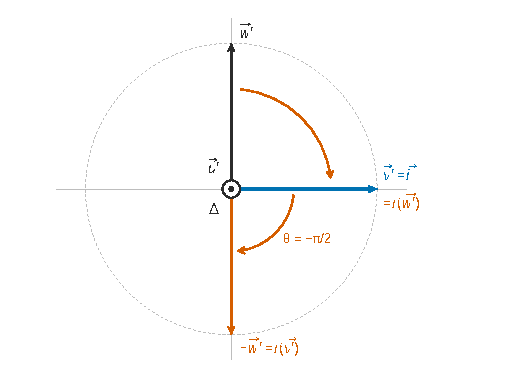
\includegraphics{figures/ex1-q10-rotation-plan-orthogonal.pdf}
\caption*{Figure 1 --- action de r dans le plan (v′, w′) orthogonal à Δ, vu depuis
la pointe de u′ : quart de tour en sens horaire, r(v′) = −w′ et r(w′) =
v′}
\end{figure}

\hypertarget{section-9}{%
\subsubsection{11.}\label{section-9}}

Soit \(P\) la matrice de passage de la base canonique à \(\mathcal{B}'\) : ses colonnes sont les coordonnées de \(\vec u\,'\), \(\vec v\,'\), \(\vec w\,'\).

Par la formule de changement de base pour un endomorphisme, \(R=PR'P^{-1}\). Comme \(P\) passe d'une base orthonormée à une autre, elle est orthogonale et \(P^{-1}=P^\top\). Donc \(R=PR'P^\top\), avec :

\equationajustee{\begin{aligned}
P&=\begin{pmatrix}0&1&0\\ \frac{1}{\sqrt2}&0&-\frac1{\sqrt2}\\ -\frac1{\sqrt2}&0&-\frac1{\sqrt2}\end{pmatrix},\\
PR'&=\begin{pmatrix}0&0&1\\ \frac1{\sqrt2}&\frac1{\sqrt2}&0\\ -\frac1{\sqrt2}&\frac1{\sqrt2}&0\end{pmatrix}.
\end{aligned}}

\equationajustee{\boxed{R=PR'P^\top=\begin{pmatrix}0&-\frac{\sqrt2}2&-\frac{\sqrt2}2\\ \frac{\sqrt2}2&\frac12&-\frac12\\ \frac{\sqrt2}2&-\frac12&\frac12\end{pmatrix}.}}

Contrôles :

\begin{itemize}
\tightlist
\item
  \(R\,\vec u\,'=\vec u\,'\) (l'axe est fixe) ;
\item
  \(\operatorname{tr}R=1\), et \(1+2\cos\theta=1\) ;
\item
  \(R\vec i=\frac{\sqrt2}{2}(\vec j+\vec k)=-\vec w\,'\), qui est bien \(r(\vec v\,')\) d'après \(R'\).
\end{itemize}

\hypertarget{section-10}{%
\subsubsection{12.}\label{section-10}}

\(R\) est orthogonale, donc \(R^\top=R^{-1}\).

\textbf{\(R^\top\) est canoniquement associée à \(r^{-1}\), la rotation d'axe \(\Delta\) (orienté par \(\vec u\)) et d'angle \(\frac\pi2\).}

\(r\) est la rotation d'angle \(-\frac\pi2\), donc \(r^4\) est la rotation d'angle \(-2\pi\). Ainsi \(r^4=\mathrm{id}\) et \(R^4=I_3\).

On a \(2025=4\times506+1\) et \(2026=4\times506+2\). D'où :

\begin{itemize}
\tightlist
\item
  \textbf{\(R^{2025}=R\) : c'est la rotation \(r\) elle-même} (axe \(\Delta\) orienté par \(\vec u\), angle \(-\frac\pi2\)) ;
\item
  \(R^{2026}=R^2\) est associée à \(r^2\), avec :
\end{itemize}

\equationajustee{R^2=\begin{pmatrix}-1&0&0\\0&0&-1\\0&-1&0\end{pmatrix}.}

Deux descriptions de \(r^2\) :

\begin{enumerate}
\def\labelenumi{\arabic{enumi}.}
\tightlist
\item
  \textbf{la rotation d'axe \(\Delta\) et d'angle \(\pi\)} (demi-tour, ou retournement d'axe \(\Delta\)) ;
\item
  \textbf{la symétrie orthogonale par rapport à la droite \(\Delta=\operatorname{Vect}(\vec j-\vec k)\)}, c'est-à-dire parallèlement au plan \(\Delta^\perp=\operatorname{Vect}(\vec i,\vec j+\vec k)\). Elle fixe \(\vec j-\vec k\) et change \(\vec i\) et \(\vec j+\vec k\) en leurs opposés, ce qu'on lit sur \(R^2\), matrice symétrique et orthogonale.
\end{enumerate}

\hypertarget{partie-d}{%
\subsection{Partie D}\label{partie-d}}

\hypertarget{section-11}{%
\subsubsection{13.}\label{section-11}}

On applique la formule de la question 3, en coordonnées \((a,b,c)\) dans \((1+X^3,X,X^2)\), et on réécrit chaque image dans \(\mathcal{B}\).

Pour \(e_1=\frac{1+X^3}{\sqrt2}\), on a \(a=\frac1{\sqrt2}\) et \(b=c=0\) :

\equationajustee{f(e_1)=\frac1{\sqrt2}(X+X^2)=\frac1{\sqrt2}e_2+\frac1{\sqrt2}e_3.}

Pour \(e_2=X^2\), on a \(c=1\) et \(a=b=0\) :

\equationajustee{\begin{aligned}
f(e_2)&=-\frac12(1+X^3)-\frac12X+\frac12X^2\\
&=-\frac{1}{\sqrt2}e_1+\frac12e_2-\frac12e_3.
\end{aligned}}

Pour \(e_3=X\), on a \(b=1\) et \(a=c=0\) :

\equationajustee{\begin{aligned}
f(e_3)&=-\frac12(1+X^3)+\frac12X-\frac12X^2\\
&=-\frac1{\sqrt2}e_1-\frac12e_2+\frac12e_3.
\end{aligned}}

En rangeant ces coordonnées en colonnes :

\equationajustee{\boxed{\operatorname{Mat}_{\mathcal{B}}(f)=\begin{pmatrix}0&-\frac{\sqrt2}2&-\frac{\sqrt2}2\\ \frac{\sqrt2}2&\frac12&-\frac12\\ \frac{\sqrt2}2&-\frac12&\frac12\end{pmatrix}=R.}}

C'est la matrice \(R\) de la question 11. Elle est orthogonale de déterminant \(1\), et \(\mathcal{B}\) est orthonormée : \(f\) est une rotation de l'espace euclidien \(H\) (orienté par \(\mathcal{B}\)).

\hypertarget{section-12}{%
\subsubsection{14.}\label{section-12}}

\textbf{Existence.} On cherche \(\mathcal{B}''=(\varepsilon_1,\varepsilon_2,\varepsilon_3)\), base de \(H\), telle que :

\equationajustee{\begin{aligned}
f(\varepsilon_1)&=\varepsilon_1,\\
f(\varepsilon_2)&=-\varepsilon_3,\\
f(\varepsilon_3)&=\varepsilon_2.
\end{aligned}}

\emph{Vecteur invariant.} Pour \(P=a(1+X^3)+bX+cX^2\), la question 3 montre que \(f(P)=P\) équivaut au système :

\equationajustee{\begin{cases}-\frac{b+c}2=a\\[2pt] a+\frac{b-c}2=b\\[2pt] a-\frac{b-c}2=c\end{cases}}

Les deux dernières équations donnent \(a=\frac{b+c}2\), la première \(a=-\frac{b+c}2\). Donc \(a=0\) et \(c=-b\), et \(\ker(f-\mathrm{id})=\operatorname{Vect}(X-X^2)\). On prend \(\varepsilon_1=X-X^2\).

\emph{Plan tourné.} On prend \(\varepsilon_2=1+X^3\) et \(\varepsilon_3=-f(\varepsilon_2)=-(X+X^2)\). Alors \(f(\varepsilon_2)=-\varepsilon_3\) par construction. Par la question 13, \(f(X)+f(X^2)=-(1+X^3)\), donc \(f(\varepsilon_3)=1+X^3=\varepsilon_2\).

\emph{Base.} Dans \((1+X^3,X,X^2)\), les coordonnées de \(\varepsilon_1,\varepsilon_2,\varepsilon_3\) forment la matrice :

\equationajustee{\begin{pmatrix}0&1&0\\1&0&-1\\-1&0&-1\end{pmatrix},\ \text{de \text{déterminant} } 2\neq0.}

C'est donc une base de \(H\), et

\equationajustee{\boxed{\begin{aligned}
\mathcal{B}''&=\big(X-X^2,\ 1+X^3,\ -X-X^2\big),\\
\operatorname{Mat}_{\mathcal{B}''}(f)&=\begin{pmatrix}1&0&0\\0&0&1\\0&-1&0\end{pmatrix}.
\end{aligned}}}

\textbf{Orthogonalité.} Les suites de coefficients sont \((0,1,-1,0)\), \((1,0,0,1)\) et \((0,-1,-1,0)\). Donc :

\equationajustee{\begin{aligned}
\varphi(\varepsilon_1,\varepsilon_2)&=0,\\
\varphi(\varepsilon_2,\varepsilon_3)&=0,\\
\varphi(\varepsilon_1,\varepsilon_3)&=-1+1=0.
\end{aligned}}

\textbf{\(\mathcal{B}''\) est orthogonale pour \(\varphi\).} Elle n'est pas normée : chaque vecteur est de norme \(\sqrt2\). Divisée par \(\sqrt2\), elle devient orthonormée et convient aussi.

Ce n'est pas un hasard du choix : toute base \(\mathcal{B}''\) qui convient est orthogonale.

\begin{itemize}
\tightlist
\item
  \(\varepsilon_1\in\ker(f-\mathrm{id})=\operatorname{Vect}(X-X^2)\).
\item
  \(f^2(\varepsilon_2)=-f(\varepsilon_3)=-\varepsilon_2\), donc \(\varepsilon_2\in\ker(f^2+\mathrm{id})\). Ce noyau est \(\operatorname{Vect}(1+X^3,X+X^2)\), plan orthogonal à \(X-X^2\).
\item
  Enfin \(\varepsilon_3=-f(\varepsilon_2)\). Pour \(v=\alpha(1+X^3)+\beta(X+X^2)\), on a \(f(v)=\alpha(X+X^2)-\beta(1+X^3)\), d'où \(\varphi(v,f(v))=2\alpha\beta-2\alpha\beta=0\).
\end{itemize}

\hypertarget{deuxiuxe8me-exercice}{%
\section{Deuxième exercice}\label{deuxiuxe8me-exercice}}

\hypertarget{partie-a-1}{%
\subsection{Partie A}\label{partie-a-1}}

\hypertarget{a-1}{%
\subsubsection{1.(a)}\label{a-1}}

L'équation \(\dfrac{x^2}{a^2}+\dfrac{y^2}{b^2}=1\) est celle d'une \textbf{ellipse} de centre \(O\), d'axes \((Ox)\) et \((Oy)\).

Ses sommets sont \((\pm a,0)\) et \((0,\pm b)\) ; c'est un cercle si \(a=b\).

Paramétrage usuel :

\equationajustee{\boxed{\begin{cases}x=a\cos t\\ y=b\sin t\end{cases}\qquad t\in[0,2\pi[.}}

\hypertarget{b-1}{%
\subsubsection{1.(b)}\label{b-1}}

L'équation \(\dfrac{x^2}{a^2}-\dfrac{y^2}{b^2}=1\) est celle d'une \textbf{hyperbole} de centre \(O\), de sommets \((\pm a,0)\), d'asymptotes \(y=\pm\frac bax\). Elle est formée de deux branches, \(x\geqslant a\) et \(x\leqslant-a\).

Paramétrages usuels :

\equationajustee{\boxed{\text{branche } x>0:\ \begin{cases}x=a\operatorname{ch}t\\ y=b\operatorname{sh}t\end{cases}\qquad\text{branche } x<0:\ \begin{cases}x=-a\operatorname{ch}t\\ y=b\operatorname{sh}t\end{cases}\qquad t\in\mathbb{R}.}}

On a \(\operatorname{ch}^2t-\operatorname{sh}^2t=1\) et \(\operatorname{ch}t\geqslant1\). Comme \(\operatorname{sh}\) est une bijection de \(\mathbb{R}\) sur \(\mathbb{R}\), chaque paramétrage décrit exactement sa branche.

\hypertarget{a-2}{%
\subsubsection{2.(a)}\label{a-2}}

La conique de foyer \(F\), de directrice \(\mathcal{D}\) et d'excentricité \(\varepsilon\) est l'ensemble des points \(M\) du plan tels que

\equationajustee{\boxed{MF=\varepsilon\, d(M,\mathcal{D})}}

où \(d(M,\mathcal{D})\) est la distance de \(M\) à \(\mathcal{D}\).

\hypertarget{b-2}{%
\subsubsection{2.(b)}\label{b-2}}

\textbf{C'est une ellipse si \(0<\varepsilon<1\), une parabole si \(\varepsilon=1\), une hyperbole si \(\varepsilon>1\).}

\hypertarget{section-13}{%
\subsubsection{3.}\label{section-13}}

On a \(|z'|=|z|\), et, pour \(z\neq0\), \(\arg z'\equiv\arg z+\theta\ [2\pi]\).

Donc \(OM'=OM\) et \((\overrightarrow{OM},\allowbreak \overrightarrow{OM'})\equiv\theta\ [2\pi]\), et \(M'=O\) si \(M=O\).

\textbf{On passe de \(M\) à \(M'\) par la rotation de centre \(O\) et d'angle \(\theta\).}

\hypertarget{partie-b-1}{%
\subsection{Partie B}\label{partie-b-1}}

\hypertarget{a-3}{%
\subsubsection{4.(a)}\label{a-3}}

\(\vec n=(\sqrt3,1)\) est normal à \(\mathcal{D}\), et \(\|\vec n\|^2=4\).

Le projeté \(M'\) est l'unique point de \(\mathcal{D}\) tel que \(\overrightarrow{MM'}\) soit colinéaire à \(\vec n\).

On écrit donc \(M'=M-t\vec n\), avec \(t\) réel tel que \(M'\in\mathcal{D}\) :

\equationajustee{\begin{aligned}
M'\in\mathcal{D}&\iff\sqrt3(x-\sqrt3t)+(y-t)=3\\
&\iff t=\frac{\sqrt3x+y-3}4.
\end{aligned}}

D'où :

\equationajustee{\boxed{\begin{aligned}
x'&=\frac{x-\sqrt3\,y+3\sqrt3}4,\\
y'&=\frac{-\sqrt3\,x+3y+3}4.
\end{aligned}}}

\hypertarget{b-3}{%
\subsubsection{4.(b)}\label{b-3}}

On a \(e^{i\pi/3}=\frac12+i\frac{\sqrt3}2\), \(e^{i\pi/6}=\frac{\sqrt3}2+\frac i2\) et \(\bar z=x-iy\). D'où :

\equationajustee{\bar z\,e^{i\pi/3}=\frac{x+\sqrt3y}2+i\,\frac{\sqrt3x-y}2.}

Par suite, avec la question 4.(a) :

\equationajustee{\begin{aligned}
z-\bar z\,e^{i\pi/3}+3e^{i\pi/6}&=\frac{x-\sqrt3y+3\sqrt3}2+i\,\frac{-\sqrt3x+3y+3}2\\
&=2(x'+iy')\\
&=2z'.
\end{aligned}}

Donc :

\equationajustee{\boxed{z'=\frac12\Big(z-\bar z\,e^{i\frac\pi3}+3e^{i\frac\pi6}\Big).}}

\hypertarget{section-14}{%
\subsubsection{5.}\label{section-14}}

On remplace \(z'\) par son expression obtenue à la question 4.(b) :

\equationajustee{\begin{aligned}
z-z'&=z-\frac12\Big(z-\bar z\,e^{i\frac\pi3}+3e^{i\frac\pi6}\Big)\\
&=\frac12 z+\frac12\bar z\,e^{i\frac\pi3}-\frac32e^{i\frac\pi6}.
\end{aligned}}

\equationajustee{\boxed{z-z'=\frac12\Big(z+\bar z\,e^{i\frac\pi3}-3e^{i\frac\pi6}\Big).}}

\hypertarget{section-15}{%
\subsubsection{6.}\label{section-15}}

D'après la question 5 :

\equationajustee{\Big|z+\bar z\,e^{i\pi/3}-3e^{i\pi/6}\Big|=2|z-z'|=2MM'.}

Comme \(M'\) est le projeté orthogonal de \(M\) sur \(\mathcal{D}\), \(MM'=d(M,\mathcal{D})\). Et \(|z|=OM\). Donc :

\equationajustee{M\in\mathcal{C}\iff OM=2\,d(M,\mathcal{D}).}

Le point \(O\) n'est pas sur \(\mathcal{D}\), car \(\sqrt3\cdot0+0\neq3\).

D'après la question 2, \textbf{\(\mathcal{C}\) est la conique de foyer \(O\), de directrice \(\mathcal{D}:\sqrt3x+y=3\) et d'excentricité \(2\) : c'est une hyperbole}, car \(2>1\).

\hypertarget{partie-c-1}{%
\subsection{Partie C}\label{partie-c-1}}

\hypertarget{section-16}{%
\subsubsection{7.}\label{section-16}}

Les vecteurs normaux à \(\mathcal{D}\) sont les \(\lambda(\sqrt3,1)\), \(\lambda\neq0\) ; ceux d'abscisse positive correspondent à \(\lambda>0\). On prend par exemple \(\vec u=\sqrt3\,\vec e_1+\vec e_2\).

Tous ont même direction et même sens que le vecteur unitaire \(\frac12(\sqrt3,1)\), qui s'écrit \(\big(\cos\frac\pi6,\sin\frac\pi6\big)\). Donc :

\equationajustee{\boxed{\alpha=(\vec e_1,\vec u)\equiv\frac\pi6\ [2\pi].}}

\hypertarget{a-4}{%
\subsubsection{8.(a)}\label{a-4}}

Soit \(z=e^{i\pi/6}Z\). Alors \(|z|=|Z|\) et \(\bar z=e^{-i\pi/6}\bar Z\), donc \(\bar z\,e^{i\pi/3}=e^{i\pi/6}\bar Z\). Il vient :

\equationajustee{\begin{aligned}
z+\bar z\,e^{i\pi/3}-3e^{i\pi/6}&=e^{i\pi/6}Z+e^{i\pi/6}\bar Z-3e^{i\pi/6}\\
&=e^{i\pi/6}(Z+\bar Z-3).
\end{aligned}}

Ce nombre a pour module \(|Z+\bar Z-3|\), puisque \(|e^{i\pi/6}|=1\). Par définition de \(\mathcal{C}'\) puis de \(\mathcal{C}\), on obtient une suite d'équivalences :

\equationajustee{\begin{aligned}
N\in\mathcal{C}'&\iff M\in\mathcal{C}\\
&\iff |z|=\big|z+\bar z\,e^{i\pi/3}-3e^{i\pi/6}\big|\\
&\iff |Z|=|Z+\bar Z-3|.
\end{aligned}}

\equationajustee{\boxed{N\in\mathcal{C}'\iff|Z|=|Z+\bar Z-3|.}}

\hypertarget{b-4}{%
\subsubsection{8.(b)}\label{b-4}}

Avec \(Z=x+iy\), on a \(Z+\bar Z-3=2x-3\), réel, et \(|Z|=\sqrt{x^2+y^2}\). Les deux membres étant positifs, l'égalité équivaut à celle de leurs carrés :

\equationajustee{\begin{aligned}
N\in\mathcal{C}'&\iff x^2+y^2=(2x-3)^2\\
&\iff x^2+y^2=4x^2-12x+9\\
&\iff 3x^2-12x-y^2+9=0.
\end{aligned}}

\equationajustee{\boxed{\mathcal{C}':\ 3x^2-12x-y^2+9=0.}}

\hypertarget{c}{%
\subsubsection{8.(c)}\label{c}}

Les équations et coordonnées sont données dans le repère \((O;\vec e_1,\vec e_2)\). On a \(3x^2-12x=3(x-2)^2-12\), donc l'équation s'écrit \(3(x-2)^2-y^2=3\), soit :

\equationajustee{(x-2)^2-\frac{y^2}{3}=1.}

\(\mathcal{C}'\) est une hyperbole de centre \(\Omega(2,0)\), avec \(a=1\) et \(b=\sqrt3\). Ses axes de symétrie sont les droites \(y=0\) et \(x=2\).

L'axe \(x=2\) ne la coupe pas, car \(-\frac{y^2}{3}=1\) est impossible. L'axe \(y=0\) la coupe en \(x-2=\pm1\).

\equationajustee{\boxed{\begin{aligned}{}&\text{centre } \Omega(2,0),\\
&\text{sommets } S_1(1,0)\ \text{et}\ S_2(3,0),\\
&\text{asymptotes } y=\sqrt3(x-2)\ \text{et}\ y=-\sqrt3(x-2).
\end{aligned}}}

Complément : \(c=\sqrt{a^2+b^2}=2\), d'où les foyers \((0,0)\) et \((4,0)\).

La directrice associée au foyer \(O\) est \(x=\frac32\), image de \(\mathcal{D}\) par la rotation de centre \(O\) et d'angle \(-\frac\pi6\).

\hypertarget{d}{%
\subsubsection{8.(d)}\label{d}}

\(G(0,3)\in\mathcal{C}'\), car \(0-0-9+9=0\). Posons \(\Phi(x,y)=3x^2-12x-y^2+9\). Alors :

\equationajustee{\begin{aligned}
\nabla\Phi(x,y)&=(6x-12,\,-2y),\\
\nabla\Phi(0,3)&=(-12,\,-6)\neq\vec 0.
\end{aligned}}

\(G\) est donc un point régulier, et la tangente en \(G\) est la droite passant par \(G\) et normale à \(\nabla\Phi(0,3)\) :

\equationajustee{\begin{aligned}{}&-12(x-0)-6(y-3)=0\\
\iff\ &2x+y-3=0.
\end{aligned}}

\equationajustee{\boxed{\mathcal{T}:\ 2x+y=3.}}

\hypertarget{a-5}{%
\subsubsection{9.(a)}\label{a-5}}

Tracé sur papier millimétré, unité 1 cm au moins (2 cm conseillé), repère \((O;\vec e_1,\vec e_2)\) dessiné et axes gradués :

\begin{itemize}
\tightlist
\item
  placer le centre \(\Omega(2,0)\) et les sommets \((1,0)\) et \((3,0)\) ;
\item
  tracer les asymptotes \(y=\pm\sqrt3(x-2)\). Elles passent par \(\Omega\) et par \((3,\pm\sqrt3)\approx(3;\pm1{,}73)\) : ce sont les diagonales du rectangle de construction \([1,3]\times[-\sqrt3,\sqrt3]\) ;
\item
  tracer la branche gauche (\(x\leqslant1\)). Elle passe par \((1,0)\), à tangente verticale, et par \(G(0,3)\) et \((0,-3)\) ;
\item
  tracer la branche droite (\(x\geqslant3\)), symétrique par rapport à la droite \(x=2\). Elle passe par \((3,0)\) et \((4,\pm3)\) ;
\item
  les branches se rapprochent des asymptotes sans les couper ;
\item
  on peut ajouter la tangente \(\mathcal{T}:y=3-2x\) en \(G\).
\end{itemize}

\begin{figure}[H]
\centering
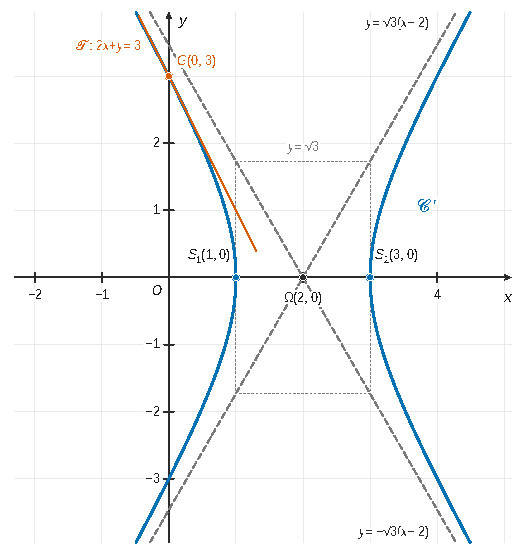
\includegraphics{figures/ex2-q9a-trace-hyperbole.pdf}
\caption*{Figure 2 --- tracé de 𝒞′ : centre Ω(2, 0), sommets S₁(1, 0) et S₂(3, 0),
rectangle de construction et asymptotes y = ±√3 (x − 2), tangente 𝒯 en
G(0, 3)}
\end{figure}

Points utiles : \(|y|=\sqrt{3\big((x-2)^2-1\big)}\). On a \(|y|=3\) pour \(x\in\{0,4\}\), et \(|y|=\sqrt{24}\approx4{,}9\) pour \(x\in\{-1,5\}\).

\hypertarget{b-5}{%
\subsubsection{9.(b)}\label{b-5}}

Par définition de \(\mathcal{C}'\), \(M\in\mathcal{C}\) si et seulement si le point \(N\) d'affixe \(Z=e^{-i\pi/6}z\) appartient à \(\mathcal{C}'\).

D'après la question 3, \(M\) d'affixe \(z=e^{i\pi/6}Z\) est l'image de \(N\) par la rotation \(\rho\) de centre \(O\) et d'angle \(\frac\pi6\).

Comme \(\rho\) est bijective, \(\mathcal{C}=\rho(\mathcal{C}')\).

\textbf{\(\mathcal{C}\) est l'image de \(\mathcal{C}'\) par la rotation de centre \(O\) et d'angle \(\alpha=\frac\pi6\).}

\begin{figure}[H]
\centering
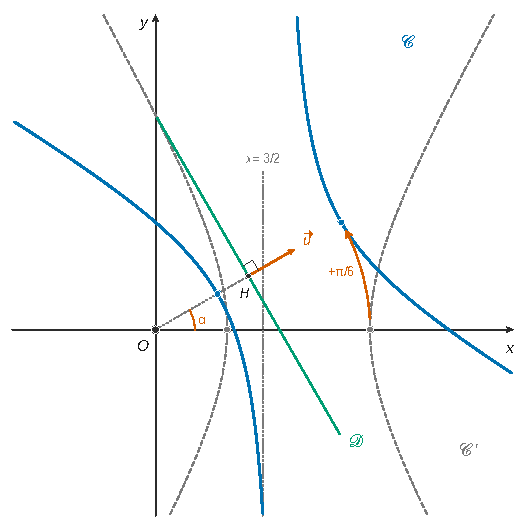
\includegraphics{figures/ex2-q9b-rotation-c-prime-c.pdf}
\caption*{Figure 3 --- la rotation de centre O et d'angle π/6 envoie 𝒞′ (gris) sur
𝒞 (bleu) et la directrice x = 3/2 sur 𝒟 ; H est le projeté de O sur 𝒟}
\end{figure}

\hypertarget{partie-d-1}{%
\subsection{Partie D}\label{partie-d-1}}

\hypertarget{section-17}{%
\subsubsection{10.}\label{section-17}}

Soit \(M(x,y,z)\in\mathcal{C}''\). Alors \(z=1\) et \(y^2=3x^2-3\), donc :

\equationajustee{\begin{aligned}
-3x^2+y^2+3z^2&=-3x^2+(3x^2-3)+3\\
&=0.
\end{aligned}}

Ainsi \(M\in S\). Tout point de \(\mathcal{C}''\) est un point de \(S\) : \textbf{\(\mathcal{C}''\subset S\).}

\hypertarget{a-6}{%
\subsubsection{11.(a)}\label{a-6}}

\(S\) a pour équation \(F(x,y,z)=0\), avec \(F(x,y,z)=-3x^2+y^2+3z^2\), fonction de classe \(C^1\) sur \({\mathbb{R}}^3\). Son gradient est :

\equationajustee{\nabla F(x,y,z)=(-6x,\,2y,\,6z).}

Le gradient est nul si et seulement si ses trois composantes sont nulles, c'est-à-dire si et seulement si \(x=y=z=0\). Il ne s'annule donc qu'en \(O\), et \(O\in S\) car \(F(0,0,0)=0\).

Un point de \(S\) est régulier si et seulement si le gradient de \(F\) y est non nul. Donc :

\equationajustee{\boxed{\text{les points \text{réguliers} de } S \text{ sont les points de } S\setminus\{O\}.}}

(\(S\) est un cône de sommet \(O\) : l'équation est homogène de degré \(2\).)

\hypertarget{b-6}{%
\subsubsection{11.(b)}\label{b-6}}

\(F(2,-3,-1)=-12+9+3=0\), donc \(J\in S\). Comme \(J\neq O\), \(J\) est régulier, avec :

\equationajustee{\nabla F(J)=(-12,-6,-6)=-6\,(2,1,1).}

Le plan tangent en \(J\) passe par \(J\) et a pour vecteur normal \((2,1,1)\) :

\equationajustee{2(x-2)+(y+3)+(z+1)=0.}

\equationajustee{\boxed{2x+y+z=0.}}

(Il passe par le sommet \(O\), comme tout plan tangent à un cône.)

\hypertarget{a-7}{%
\subsubsection{12.(a)}\label{a-7}}

L'identité se vérifie en développant :

\equationajustee{\begin{aligned}
(2x-\sqrt2z)(2x+\sqrt2z)&=4x^2-2z^2,\\
x^2+y^2+z^2-(4x^2-2z^2)&=-3x^2+y^2+3z^2.
\end{aligned}}

Pour un point de \(P_\lambda\), on a \(2x+\sqrt2z=\lambda\). On raisonne par équivalence :

\equationajustee{\begin{aligned}
M\in{\mathcal{C}}_\lambda&\iff\begin{cases}2x+\sqrt2z=\lambda\\ x^2+y^2+z^2-\lambda(2x-\sqrt2z)=0\end{cases}\\
&\iff\begin{cases}2x+\sqrt2z=\lambda\\ (x-\lambda)^2+y^2+\big(z+\frac{\lambda}{\sqrt2}\big)^2=\frac32\lambda^2.\end{cases}
\end{aligned}}

\emph{Cas \(\lambda\neq0\).} La seconde équation est celle de la sphère \(\Sigma_\lambda\) de centre \(\Omega_\lambda=\big(\lambda,0,-\frac\lambda{\sqrt2}\big)\) et de rayon \(\rho_\lambda=|\lambda|\sqrt{\frac32}>0\).

Or \(2\lambda+\sqrt2\cdot\big(-\frac{\lambda}{\sqrt2}\big)=\lambda\), donc \(\Omega_\lambda\in P_\lambda\). Un plan passant par le centre d'une sphère la coupe selon un grand cercle. \textbf{\({\mathcal{C}}_\lambda\) est le cercle de \(P_\lambda\) de centre \(\Omega_\lambda\) et de rayon \(\frac{\sqrt6}{2}|\lambda|\).}

\emph{Cas \(\lambda=0\).} La seconde équation impose \(x=y=z=0\), et \(O\in P_0\). Donc \({\mathcal{C}}_0=\{O\}\), cercle réduit à un point.

\equationajustee{\boxed{\begin{aligned}{}&\lambda\neq0:\ {\mathcal{C}}_\lambda \text{ est un cercle de rayon } \tfrac{\sqrt6}{2}|\lambda|,\\
&\lambda=0:\ {\mathcal{C}}_0=\{O\}.
\end{aligned}}}

\textbf{Remarque sur l'énoncé.} L'alternative « vide ou cercle » est inexacte : \({\mathcal{C}}_\lambda\) n'est jamais vide, et pour \(\lambda=0\) il est réduit au point \(O\) (cercle de rayon nul). On a démontré le résultat sous cette forme corrigée.

\hypertarget{b-7}{%
\subsubsection{12.(b)}\label{b-7}}

\textbf{Non.} Si \(S\) était de révolution d'axe \(A\), ses sections par les plans orthogonaux à \(A\) seraient des cercles \textbf{centrés sur \(A\)}.

Ici, les plans \(P_\lambda\) sont tous orthogonaux à \(\vec n=(2,0,\sqrt2)\).

Mais les centres \(\Omega_\lambda=\lambda\big(1,0,-\frac1{\sqrt2}\big)\) sont sur la droite passant par \(O\) et dirigée par \((\sqrt2,0,-1)\). Cette droite n'est pas colinéaire à \(\vec n\), puisque \((\sqrt2,0,-1)\cdot(2,0,\sqrt2)=\sqrt2\neq0\).

Les cercles \({\mathcal{C}}_\lambda\) ne sont donc pas centrés sur une droite orthogonale à leurs plans. L'existence de cette famille de sections circulaires parallèles ne permet pas de conclure que \(S\) est de révolution.

\begin{figure}[H]
\centering
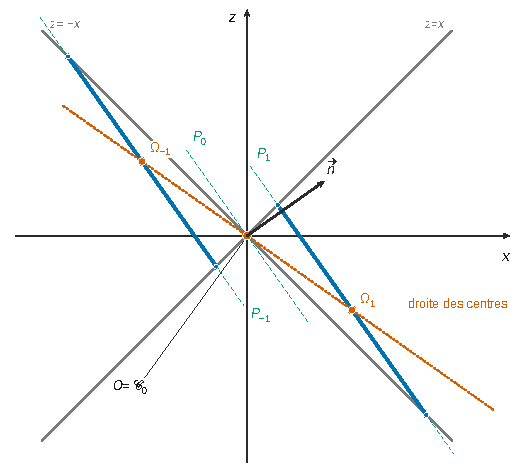
\includegraphics{figures/ex2-q12b-sections-circulaires-coupe.pdf}
\caption*{Figure 4 --- coupe par le plan y = 0 : S y laisse les droites z = ±x,
chaque 𝒞\_λ un diamètre (en bleu) ; les centres Ω\_λ sont sur une droite
non colinéaire à n = (2, 0, √2)}
\end{figure}

Remarque : les sections de \(S\) par les plans \(x=x_0\neq0\) sont les ellipses \(y^2+3z^2=3x_0^2\), non circulaires, donc \(S\) n'est pas de révolution d'axe \((Ox)\). Établir que \(S\) n'est de révolution autour d'aucun axe relèverait de la classification des quadriques, hors programme en PT ; la question ne le demande pas.

\hypertarget{section-18}{%
\subsubsection{13.}\label{section-18}}

Un point de \(\mathcal{C}''\) vérifie \(3x^2=3+y^2\geqslant3\), donc \(|x|\geqslant1\). Ainsi :

\equationajustee{\mathcal{C}''_+=\{(x,y,1)\ :\ 3x^2-y^2=3,\ x\geqslant1\}.}

Un point \(M(x,y,z)\) appartient à \(\Sigma\) si et seulement s'il existe \(M_0(x_0,y_0,1)\in\mathcal{C}''_+\) sur le même cercle d'axe \((Ox)\). Cela signifie \(x=x_0\) et \(y^2+z^2=y_0^2+1\).

\begin{itemize}
\tightlist
\item
  Si \(M\in\Sigma\) : \(x=x_0\geqslant1\) et \(y^2+z^2=y_0^2+1=(3x^2-3)+1=3x^2-2\).
\item
  Réciproquement, supposons \(x\geqslant1\) et \(y^2+z^2=3x^2-2\).
  Le point \(M_0=\big(x,\sqrt{3x^2-3},1\big)\) est bien défini (\(3x^2-3\geqslant0\)) et appartient à \(\mathcal{C}''_+\). Il vérifie \(y_0^2+1=3x^2-2=y^2+z^2\), donc \(M\in\Sigma\).
\end{itemize}

\equationajustee{\boxed{\Sigma:\quad 3x^2-y^2-z^2=2\quad\text{et}\quad x\geqslant1.}}

La condition \(x\geqslant1\) est indispensable.

L'équation seule décrit les deux nappes d'un hyperboloïde de révolution à deux nappes (\(|x|\geqslant\sqrt{2/3}\)), alors que \(\Sigma\) n'en est que la partie \(x\geqslant1\). Sa méridienne est \(r=\sqrt{3x^2-2}\) pour \(x\geqslant1\) ; elle part du point \((x,r)=(1,1)\).

\end{document}
